\chapter{Matematyczne podstawy}
% =======================================================
\epigraph{\textit{„Matematyka jest alfabetem, za pomocą którego Bóg opisał wszechświat.”}}{--- Galileusz}

\section{Układy współrzędnych i ich transformacje}

Planowanie lotu i wyznaczanie trajektorii w otwartej przestrzeni w pierwszej kolejności wymaga określenia zadowalającego sposobu ułożenia siatki, po której poruszać się będzie statek. Systemy pozycjonowania (takie jak GPS) dostarczają dane w układzie absolutnym (geodezyjnym/sferycznym), które najczęściej muszą być przez algorytmy robotyczne przeliczone na układy lokalne (płaskie/kartezjańskie). 

Rozważania przedstawione w tej sekcji, opisujące naturę systemów odniesienia oraz matematyczne ramy przejścia z elipsoidy na płaszczyznę, opierają się m.in. na opracowaniu J. Lamparskiego\footnote{Lamparski J., \textit{Układy współrzędnych stosowane w Polsce i ich relacje względem globalnego układu WGS84}, NAVI sp. z o.o., 1998. Dostęp online: \href{https://www.navi.pl/katalog/0/113/uklady_wspolrzednych.html}{navi.pl}}.

% -------------------------------------------------------

\subsection{Układy przestrzenne: Od kuli do elipsoidy (WGS84)}

Aby precyzyjnie kontrolować drona, musimy najpierw zrozumieć, w jaki sposób opisujemy pozycję na Ziemi. Ewolucja systemów nawigacyjnych przebiegała od uproszczonych modeli idealnej kuli aż po precyzyjne elipsoidy obrotowe.

\begin{figure}[ht]
    \centering
    
\includegraphics[width=0.55\textwidth]{figures/uw_1.png}
    \caption{Układ współrzędnych geograficznych na wyidealizowanej kuli.}
    \label{fig:geo_uklad}
\end{figure}
\subsubsection{Model idealnej kuli}
Jak zilustrowano na Rysunku \ref{fig:geo_uklad}, najprostszą formą opisu położenia dowolnego obiektu jest \textbf{układ współrzędnych geograficznych}. Model ten zakłada, że Ziemia jest idealną kulą. Położenie wyznacza się w nim za pomocą dwóch kątów określających geocentryczny kierunek względem przyjętych osi. Znajdujące się na rysunku zmienne oznaczają:
\begin{itemize}
    \item \textbf{$O$ (Środek kuli):} Geometryczny środek sfery, stanowiący początek układu współrzędnych.
    \item \textbf{$B$ oraz $B_1$ (Bieguny):} Punkty przecięcia osi obrotu Ziemi z powierzchnią sfery. Symbol $B$ oznacza \textbf{Biegun Północny}, natomiast $B_1$ oznacza \textbf{Biegun Południowy}. Prosta przechodząca przez punkty $B-O-B_1$ definiuje oś obrotu kuli ziemskiej.
    \item \textbf{$R$ oraz $R_1$ (Płaszczyzna Równika):} Punkty skrajne wyznaczające na rzucie płaszczyznę równika ziemskiego (koła wielkiego prostopadłego do osi obrotu $B-B_1$). Płaszczyzna ta dzieli kulę na półkulę północną (z biegunem $B$) i południową (z biegunem $B_1$).
    \item \textbf{Południk początkowy:} Półokrąg wielki łączący bieguny $B$ i $B_1$, przyjęty umownie jako odniesienie zerowe (odpowiednik południka Greenwich), od którego mierzony jest kąt długości geograficznej.
    \item \textbf{$P$ (Punkt przestrzenny):} Dowolny analizowany punkt (obiekt, dron, stacja pomiarowa) zlokalizowany na powierzchni kuli.
    \item \textbf{$-R-$ (Promień):} Odcinek łączący środek kuli $O$ z punktem $P$, reprezentujący promień sfery (wektor wodzący punktu).
    \item \textbf{$\varphi$ (Szerokość geograficzna):} Kąt pionowy mierzony w płaszczyźnie południka punktu $P$, zawarty pomiędzy płaszczyzną równika ($R-R_1$) a promieniem wodzącym $OP$. Strzałka ze znakiem \textbf{„$+$”} wskazuje kierunek dodatni (na północ, od $0^\circ$ do $+90^\circ$ w punkcie $B$).
    \item \textbf{$\lambda$ (Długość geograficzna):} Kąt poziomy (dwuścienny) mierzony w płaszczyźnie równika, zawarty pomiędzy południkiem początkowym a południkiem przechodzącym przez punkt $P$. Strzałka ze znakiem \textbf{„$+$”} wskazuje kierunek dodatni (na wschód, od $0^\circ$ do $+180^\circ$).
    \item \textbf{$\delta$ (Odległość biegunowa / Kąt biegunowy):} Kąt zawarty między osią obrotu sfery (kierunkiem ku biegunowi północnemu $B$) a promieniem wodzącym $OP$. W geodezji i astronomii wielkość ta nazywana jest \textit{odległością biegunową} (ang. \textit{polar distance} lub \textit{colatitude}). Stanowi ona dopełnienie szerokości geograficznej do kąta prostego:
    \begin{equation*}
        \delta = 90^\circ - \varphi
    \end{equation*}
\end{itemize}
\subsubsection{Model elipsoidy}
Model idealnej kuli sprawdzał się w dawnej nawigacji morskiej. Jednak wraz z rozwojem inżynierii oraz systemów nawigacji satelitarnej (takich jak GPS), dokładność rzędu dziesiątek metrów okazała się niewystarczająca. Ze względu na działanie sił odśrodkowych wynikających z ruchu wirowego, Ziemia jest spłaszczona na biegunach i rozszerzona na równiku. Wymusiło to przejście na \textbf{układ współrzędnych elipsoidalnych}.

\begin{figure}[ht]
    \centering
    
\includegraphics[width=0.55\textwidth]{figures/uw_2.png}
    \caption{Układ współrzędnych elipsoidalnych w rzucie przestrzennym.}
    \label{fig:elip_uklad}
\end{figure}

Jak przedstawia Rysunek \ref{fig:elip_uklad}, powierzchnią odniesienia matematycznego nie jest już kula, lecz elipsoida obrotowa. Ta zmiana geometrii wprowadza do obliczeń nowe wartości i definicje:
\begin{itemize}
    \item \textbf{$O$ (Środek układu):} Geometryczny środek elipsoidy obrotowej, stanowiący początek kartezjańskiego układu współrzędnych $(0,0,0)$ (w modelach globalnych, takich jak WGS84, pokrywa się ze środkiem masy Ziemi).
    \item \textbf{$x, y, z$ (Osie kartezjańskie):} Prawoskrętny układ osi przestrzennych. Oś $z$ stanowi oś obrotu elipsoidy, oś $x$ leży w płaszczyźnie południka zerowego i równika, a oś $y$ dopełnia układ w płaszczyźnie równika pod kątem $90^\circ$. Pogrubione linie przerywane wskazują rzut współrzędnych kartezjańskich $(x, y, z)$ punktu $P$.
    \item \textbf{$N$ oraz $S$ (Bieguny):} Punkty przecięcia osi obrotu $z$ z powierzchnią elipsoidy. Oznaczają odpowiednio \textbf{Biegun Północny} (\textit{North}) oraz \textbf{Biegun Południowy} (\textit{South}).
    \item \textbf{$\omega$ (Prędkość kątowa):} Wektor prędkości kątowej określający ruch wirowy Ziemi (obrót elipsoidy wokół osi biegunowej $z$).
    \item \textbf{$a$ oraz $b$ (Półosie elipsoidy):} Podstawowe parametry geometryczne elipsoidy obrotowej:
    \begin{itemize}
        \item $a$ -- \textbf{duża półoś} (promień równikowy, mierzony w płaszczyźnie $xy$),
        \item $b$ -- \textbf{mała półoś} (promień biegunowy, mierzony wzdłuż osi obrotu $z$ od środka $O$ do bieguna $N$).
    \end{itemize}
    \item \textbf{$P$ (Punkt na elipsoidzie):} Analizowany punkt położony bezpośrednio na powierzchni elipsoidy odniesienia (z tego powodu wysokość elipsoidalna $H$ na tej rycinie nie występuje, gdyż wynosi $H=0$).
    \item \textbf{$\mathbf{n}$ (Wektor normalny):} Jednostkowy wektor prostopadły do powierzchni stycznej do elipsoidy w punkcie $P$. Linia przechodząca przez ten wektor to \textbf{normalna elipsoidy w punkcie $P$}.
    \item \textbf{$B = B_0$ (Równik):} Płaszczyzna równika elipsoidy (równoleżnik zerowy o szerokości geodezyjnej $B_0 = 0^\circ$).
    \item \textbf{$B = B_p$ oraz $B_p$ (Szerokość geodezyjna):} Krzywa $B=B_p$ to równoleżnik przechodzący przez punkt $P$. Kąt $B_p$ to \textbf{szerokość geodezyjna} punktu $P$, mierzona w płaszczyźnie południka między płaszczyzną równika a kierunkiem normalnej elipsoidy.
    \item \textbf{$L = L_0$ (Południk początkowy / zerowy):} Płaszczyzna południka odniesienia (dla którego długość geodezyjna wynosi $L_0 = 0^\circ$).
    \item \textbf{$L = L_p$ oraz $L_p$ (Długość geodezyjna):} Krzywa $L=L_p$ to południk przechodzący przez punkt $P$ i łączący bieguny $N$ i $S$. Kąt $L_p$ to \textbf{długość geodezyjna} punktu $P$, mierzona w płaszczyźnie równika od południka zerowego do południka punktu $P$.
    \item \textbf{$p$ (Odległość biegunowa / Colatitude):} Kąt zawarty pomiędzy osią obrotu elipsoidy (kierunkiem bieguna północnego $N$) a kierunkiem wyznaczonym przez punkt $P$. Podobnie jak na sferze, kąt ten jest dopełnieniem szerokości geodezyjnej do kąta prostego:
    \begin{equation*}
        p = 90^\circ - B_p
    \end{equation*}
\end{itemize}
\subsubsection{Model WGS84}
Drony i współczesne systemy GNSS bazują powszechnie na światowym standardzie odniesienia \textbf{WGS84} (\textit{World Geodetic System 1984}). Standard ten to nic innego, jak globalnie ujednolicona elipsoida, która przyjmuje dłuższą półoś na poziomie dokładnie $a = 6\,378\,137$ m. Współrzędne można wyrażać w niej kątowo (geodezyjnie: $B, L, H$), ale do obliczeń wektorowych drony korzystają z jej rzutu kartezjańskiego.

\begin{figure}[ht]
    \centering
    
\includegraphics[width=0.55\textwidth]{figures/uw_3.png}
    \caption{Geocentryczny układ współrzędnych ortokartezjańskich WGS84.}
    \label{fig:wgs84_uklad}
\end{figure}

Rysunek \ref{fig:wgs84_uklad} przedstawia trójwymiarowy układ kartezjański wpisany w elipsoidę systemu WGS84. Parametry osi zdefiniowane są w sposób uniwersalny dla całego globu:
\begin{itemize}
    \item \textbf{Centrum środka mas Ziemi $(0,0,0)$:} 
    Początek układu współrzędnych ortokartezjańskich (zaznaczony czarnym punktem w centrum elipsoidy). Pokrywa się on ściśle z fizycznym środkiem masy całej Ziemi (wliczając w to masę oceanów oraz atmosfery). Dzięki temu układ WGS84 jest układem \textbf{geocentrycznym}, co umożliwia precyzyjny opis orbit satelitów systemu GPS na bazie praw grawitacji Newtona.

    \item \textbf{Oś $Z_{\text{WGS84}}$ oraz CTP (\textit{Conventional Terrestrial Pole}):} 
    Pionowa oś układu, skierowana wzdłuż osi obrotu Ziemi w stronę bieguna północnego. Zgodnie z etykietą na rysunku, jej kierunek definiowany jest przez umowny biegun ziemski \textbf{CTP (1984)} (\textit{Conventional Terrestrial Pole}). Jest to uśredniony w czasie (dla epoki 1984.0) biegun obrotu wyznaczony przez międzynarodowe służby geodezyjne, co eliminuje wpływ zjawiska tzw. wędrówki bieguna (ruchu precesyjno-nutacyjnego i okresowych drgań osi Ziemi).

    \item \textbf{Oś $X_{\text{WGS84}}$ oraz Południk zerowy BIH (1984):} 
    Pozioma oś leżąca w płaszczyźnie równika. Jej kierunek wyznacza prosta przecięcia płaszczyzny równika z płaszczyzną \textbf{południka zerowego zdefiniowanego przez BIH} (\textit{Bureau International de l'Heure}) w epoce 1984.0 (obecnie jest to tzw. południk odniesienia IERS -- \textit{IERS Reference Meridian}). Warto odnotować, że południk ten przebiega około $102$ metry na wschód od historycznego, astronomicznego południka Greenwich. Wzdłuż tej osi długość geodezyjna wynosi $L = 0^\circ$, a szerokość $B = 0^\circ$.

    \item \textbf{Oś $Y_{\text{WGS84}}$:} 
    Oś leżąca w płaszczyźnie równika, prostopadła do osi $X_{\text{WGS84}}$ i $Z_{\text{WGS84}}$. Została skierowana w stronę długości geograficznej $90^\circ\text{ E}$ (na wschód), uzupełniając trójkę wektorów bazowych tak, aby tworzyły one \textbf{prawoskrętny, trójwymiarowy ortogonalny (prostokątny) układ współrzędnych}.

    \item \textbf{Siatka elipsoidy na rysunku (płaszczyzny bazowe):}
    \begin{itemize}
        \item \textbf{Płaszczyzna równika ($X_{\text{WGS84}} - Y_{\text{WGS84}}$):} Elipsa pozioma przechodząca przez środek układu reprezentuje równik elipsoidy WGS84, na którym szerokość geodezyjna wynosi $B = 0^\circ$.
        \item \textbf{Łuk południka zerowego ($X_{\text{WGS84}} - Z_{\text{WGS84}}$):} Pionowy łuk łączący biegun $Z_{\text{WGS84}}$ z osią $X_{\text{WGS84}}$ reprezentuje południk początkowy ($L = 0^\circ$).
        \item \textbf{Łuk południka $90^\circ\text{ E}$ ($Y_{\text{WGS84}} - Z_{\text{WGS84}}$):} Pionowy łuk prostopadły do południka zerowego, wyznaczający kierunek ćwiartkowy wschodni.
    \end{itemize}
\end{itemize}

Przejście z układu elipsoidalnego ($B, L, H$) do pełnego układu kartezjańskiego 3D ($X, Y, Z$) wymaga użycia pierwszego mimośrodu elipsoidy ($e$). Relację tę (rzutowanie na układ geocentryczny) opisują analityczne wzory:

\begin{align}
    X &= (N + H) \cos B \cos L \\
    Y &= (N + H) \cos B \sin L \\
    Z &= [N(1 - e^2) + H] \sin B
\end{align}

gdzie wspomniany już wcześniej promień krzywizny $N$ dany jest wzorem:
\begin{equation}
    N = \frac{a}{\sqrt{1 - e^2 \sin^2 B}}
\end{equation}

Rozwiązanie problemu odwrotnego (wyznaczenie szerokości i długości ze współrzędnych kartezjańskich $X, Y, Z$) jest zagadnieniem znacznie bardziej złożonym i na drodze obliczeniowej wymaga implementacji algorytmów iteracyjnych, przybliżających wartość kąta $B$ aż do osiągnięcia ustalonego progu zbieżności.

\subsection{Układy płaskie (Odwzorowania Kartograficzne)}
Choć globalny system GPS zapewnia dokładność pozycjonowania 3D, z punktu widzenia projektowania map ortofotomap (fotogrametria z dronów) oraz matematycznego planowania trajektorii skanowania pól – znacznie wygodniej jest operować na standardowym układzie płaskim w metrach. W tym celu korzysta się z procedur zwanych odwzorowaniami kartograficznymi, które pozwalają „rozwinąć” trójwymiarową sferę na dwuwymiarowy arkusz $x, y$. 

W geodezji najcenniejsze są odwzorowania wiernokątne (np. Gaussa-Krügera lub Merkatora), które choć zniekształcają (w minimalnym stopniu) długości, to nie zniekształcają w ogóle kątów na mapie, co jest kluczowe dla poprawności nawigacyjnej i obliczania azymutów. 

\subsubsection{Układ NED}
W kontekście programowania autonomicznych misji BSP, nie używamy skomplikowanych państwowych odwzorowań geodezyjnych na duże dystanse (jak polski system PUGK'65 czy PL-1992). Loty dronów trwają stosunkowo krótko i w małym promieniu operacyjnym. Dlatego zamiast odwzorowań walcowych wprowadzamy tzw. \textbf{Lokalny System Kartezjański}, potocznie określany w literaturze lotniczej mianem układu \textbf{NED} (\textit{North, East, Down}).

\begin{figure}[ht]
    \centering
    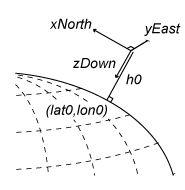
\includegraphics[scale=1]{figures/ned_system.png}
    \caption{Układ współrzędnych North-East-Down (NED).}
    \label{fig:elip_uklad}
\end{figure}
Układ ten budowany jest „w locie” i opiera się na umieszczeniu płaszczyzny stycznej do kuli ziemskiej dokładnie w punkcie, w którym znajduje się baza operacyjna statku ($X=0, Y=0, Z=0$). Osie układu definiuje się następująco:
\begin{itemize}
    \item Oś $X$ (\textit{North}) skierowana jest idealnie wzdłuż lokalnego południka geograficznego na północ geograficzną.
    \item Oś $Y$ (\textit{East}) skierowana jest wzdłuż lokalnego równoleżnika na wschód geograficzny.
    \item Oś $Z$ (\textit{Down}) skierowana jest ortogonalnie w dół (w stronę środka masy Ziemi), domykając prawoskrętny układ współrzędnych. Wynika z tego, że ujemne wartości na osi Z będą oznaczać wzrost wysokości statku nad ziemią (pułap $H_{alt} = -Z_{ned}$).
\end{itemize}

% -------------------------------------------------------

\subsection{Przykład praktyczny: Translacje za pomocą przybliżenia sferycznego}
Przy założeniu relatywnie krótkich misji (poniżej $10$ km długości wektora), krzywiznę elipsoidy w procedurach inżynierskich drona można zminimalizować do promienia kuli $R = 6\,378\,137$ m, co pozwala zredukować skomplikowane przekształcenia tensorowe Gaussa do bardzo prostego układu trygonometrycznego.

W niniejszym kursie algorytmika Pythona używa matematycznego wzoru do natychmiastowego przetłumaczenia zadanego przesunięcia w płaskim układzie kartezjańskim (np. "przesuń cel o $\Delta North$ oraz $\Delta East$ metrów") z powrotem na język globalnego modułu satelitarnego WGS84:

\begin{lstlisting}[language=Python, caption=Przeliczanie przesunięcia metrycznego w układzie NED na współrzędne GPS (w oparciu o promień kuli)]
def get_location_meters(original_location, d_north, d_east):
    earth_radius = 6378137.0
    
    # Krok 1: Wyliczenie offsetu katowego (w radianach)
    d_lat = d_north / earth_radius
    
    # Wspolrzedna East wymaga doliczenia funkcji 'cos', poniewaz obwody 
    # rownoleznikow zawezaja sie wraz ze zblizaniem sie do biebunow Ziemi
    d_lon = d_east / (earth_radius * math.cos(math.pi * original_location.lat / 180.0))
    
    # Krok 2: Zamiana radianow na stopnie dziesietne (decimal degrees)
    new_lat = original_location.lat + (d_lat * 180.0 / math.pi)
    new_lon = original_location.lon + (d_lon * 180.0 / math.pi)
    
    return LocationGlobalRelative(new_lat, new_lon, original_location.alt)
\end{lstlisting}

Podobne uproszczenia (przybliżenie Płaskiej Ziemi) stosujemy, obliczając najkrótszą odległość euklidesową (w metrach) pomiędzy dwoma punktami GPS. Znając z geometrii definicję miary Pitagorasa $\Delta d = \sqrt{\Delta x^2 + \Delta y^2}$, musimy jedynie odpowiednio wylistować długości łuków, korzystając ze stałego przelicznika $1^\circ \approx 111,319.5$ metrów. 
\begin{lstlisting}[language=Python, caption=Wyznaczanie odległości euklidesowej z układu geodezyjnego]
def get_distance_metres(loc1, loc2):
    """
    Krotki algorytm obliczania odleglosci euklidesowej w metrach. 
    Wzor wykorzystuje stala zamiane stopni na metry.
    """
    d_lat = loc2.lat - loc1.lat
    d_lon = loc2.lon - loc1.lon
    return math.sqrt((d_lat**2) + (d_lon**2)) * 1.113195e5
\end{lstlisting}
Tak przedstawiona dualność opisu trajektorii pozwala algorytmice drona realizować misje na geometrycznie doskonałej, dwuwymiarowej tablicy kartezjańskiej (co wybitnie sprawdza się m.in. w implementacji algorytmów Sweep-Line i Kosiarki z modułu CPP), jednocześnie gwarantując wykonanie poprawnego, wolnego od dryfu satelitarnego toru przelotu w świecie rzeczywistym.




\section{Krzywe parametryczne w modelowaniu trajektorii}

W klasycznym podejściu nawigacyjnym trajektorię lotu definiuje się jako uporządkowany ciąg punktów orientacyjnych (ang. \textit{waypoints}) $W = \{w_1, w_2, \dots, w_m\} \subset \mathbb{R}^3$, połączonych odcinkami prostoliniowymi. Choć metoda ta sprawdza się w misjach transportowych na dużych wysokościach, posiada fundamentalne wady w sterowaniu autonomicznym:
\begin{itemize}
    \item \textbf{Brak gładkości ($C^0$):} W węzłach $w_i$ wektor prędkości doznaje skokowej zmiany kierunku. Realizacja takiego ruchu przez układ fizyczny wymagałaby nieskończenie dużych sił (przyspieszeń), co w praktyce wymusza wyhamowanie statku niemal do zera przed każdym zakrętem.
    \item \textbf{Nieoptymalne zużycie energii:} Ciągłe cykle hamowania i przyspieszania drastycznie skracają czas pracy akumulatorów LiPo.
\end{itemize}

Rozwiązaniem tego problemu jest modelowanie toru ruchu za pomocą \textbf{krzywych parametrycznych klasy co najmniej $C^2$} (dwukrotnie różniczkowalnych w sposób ciągły):
\begin{equation}
    \mathbf{r}(t) = \begin{bmatrix} x(t) \\ y(t) \\ z(t) \end{bmatrix}, \quad t \in [t_0, t_k]
\end{equation}
gdzie parametr $t$ utożsamiamy najczęściej z czasem fizycznym. Taki opis pozwala na bezpośrednie wyznaczenie wektora prędkości $\mathbf{v}(t) = \mathbf{\dot{r}}(t)$ oraz wektora przyspieszenia $\mathbf{a}(t) = \mathbf{\ddot{r}}(t)$, co umożliwia kontrolerom lotu płynne sterowanie ciągiem i kątami przechylenia statku.


\subsection{Krzywe w przestrzeni 2D}

Rozważmy ruch w płaszczyźnie poziomej przy założeniu stałego pułapu ($z(t) = \text{const}$, $v_z = 0$). Niech $\mathbf{r}(t) = [x(t), y(t)]^T$ będzie krzywą płaską. 

\subsubsection{Krzywizna a ograniczenia fizyczne}
Kluczowym pojęciem analizy trajektorii jest jej \textbf{krzywizna} $\kappa(t)$, mierząca tempo zmiany kierunku wektora stycznego:
\begin{equation}
    \kappa(t) = \frac{|\dot{x}\ddot{y} - \dot{y}\ddot{x}|}{(\dot{x}^2 + \dot{y}^2)^{3/2}} = \frac{\|\mathbf{\dot{r}}(t) \times \mathbf{\ddot{r}}(t)\|}{\|\mathbf{\dot{r}}(t)\|^3}
\end{equation}
Z mechaniki newtonowskiej wynika, że ruch po krzywej o krzywiźnie $\kappa(t)$ z prędkością skalarną $v(t) = \|\mathbf{\dot{r}}(t)\|$ generuje przyspieszenie dośrodkowe:
\begin{equation}
    a_n(t) = v^2(t) \cdot \kappa(t)
\end{equation}
Ponieważ maksymalny kąt przechylenia drona (ang. \textit{tilt angle}) jest ograniczony parametrami konstrukcyjnymi i stabilnością aerodynamiczną, maksymalne dopuszczalne przyspieszenie boczne wynosi $a_{\max} = g \tan(\theta_{\max})$. Wprowadza to twarde ograniczenie na prędkość w zakręcie:
\begin{equation}
    v(t) \le \sqrt{\frac{a_{\max}}{\kappa(t)}}
\end{equation}
W punktach o dużej krzywiźnie $\kappa$ (ostre skręty) dron musi zredukować prędkość, natomiast na odcinkach o $\kappa \approx 0$ może poruszać się z prędkością maksymalną.

\subsubsection{Przykłady krzywych analitycznych}

W module \texttt{02\_fizyka\_i\_matematyka} (skrypt \texttt{03\_parametric\_shapes.py}) zaimplementowano trzy reprezentatywne geometrie:

\paragraph{1. Okrąg (Krzywa o stałej krzywiźnie):}
Najprostsza krzywa zamknięta o stałej krzywiźnie $\kappa = \frac{1}{R}$:
\begin{equation}
    \begin{cases}
        x(t) = R \cos(\omega t) - R \\
        y(t) = R \sin(\omega t)
    \end{cases}, \quad t \in \left[0, \frac{2\pi}{\omega}\right]
\end{equation}
Przesunięcie o $-R$ na osi $x$ zostało zastosowane w celu zapewnienia warunku początkowego $\mathbf{r}(0) = [0, 0]^T$, dzięki czemu dron rozpoczyna manewr bezpośrednio z punktu zawisu. Prędkość i przyspieszenie wynoszą odpowiednio:
\begin{align}
    \mathbf{v}(t) &= [-R\omega \sin(\omega t), R\omega \cos(\omega t)]^T, \quad \|\mathbf{v}(t)\| = R\omega = \text{const} \\
    \mathbf{a}(t) &= [-R\omega^2 \cos(\omega t), -R\omega^2 \sin(\omega t)]^T, \quad \|\mathbf{a}(t)\| = R\omega^2 = \text{const}
\end{align}
Stałość modułu przyspieszenia oznacza, że dron utrzymuje stały kąt przechyłu (Roll) przez cały czas trwania manewru.

\paragraph{2. Lemniskata Gerono (Ósemka):}
Krzywa w kształcie cyfry 8, stosowana powszechnie w procedurach kalibracji magnetometru (kompasu) BSP:
\begin{equation}
    \begin{cases}
        x(t) = A \sin(\omega t) \\
        y(t) = A \sin(\omega t)\cos(\omega t) = \frac{A}{2} \sin(2\omega t)
    \end{cases}, \quad t \in \left[0, \frac{2\pi}{\omega}\right]
\end{equation}
Krzywizna lemniskaty zmienia znak przy przejściu przez punkt węzłowy $(0,0)$, co wymaga od kontrolera lotu płynnego przejścia z przechyłu w lewo do przechyłu w prawo (inwersja wektora siły dośrodkowej).

\paragraph{3. Kardioida (Krzywa o zmiennej dynamice):}
Krzywa o równaniu wykorzystującym sumę harmonicznych, generująca kształt serca:
\begin{equation}
    \begin{cases}
        x(t) = 16A \sin^3(\omega t) \\
        y(t) = A \big(13\cos(\omega t) - 5\cos(2\omega t) - 2\cos(3\omega t) - \cos(4\omega t)\big)
    \end{cases}
\end{equation}
Trajektoria ta posiada ostrze (punkt osobliwy, w którym $\mathbf{\dot{r}}(t) \to 0$ przy zbliżaniu się do szpica), co stanowi doskonały poligon testowy dla algorytmów sprawdzających zachowanie pętli sterowania przy gwałtownych zmianach zwrotu wektora prędkości.

\subsubsection{Dyskretyzacja i filtracja geometryczna w kodzie}
Komputer pokładowy drona operuje w czasie dyskretnym z częstotliwością $f = \frac{1}{\Delta t}$. Ciągła krzywa $\mathbf{r}(t)$ jest próbkowana do postaci zbioru punktów węzłowych $\mathbf{P}_k = \mathbf{r}(k \Delta t)$ dla $k = 0, 1, \dots, N$. 

W skrypcie \texttt{03\_parametric\_shapes.py} zaimplementowano \textbf{pętlę nadążną z tolerancją promienia akceptacji} $r_{\text{tol}}$:
\begin{equation}
    \|\mathbf{r}_{\text{drone}} - \mathbf{P}_k\| \le r_{\text{tol}} \implies k \leftarrow k + 1
\end{equation}
Ustawienie $r_{\text{tol}} \approx 2.0\text{ m}$ działa jak mechaniczny filtr dolnoprzepustowy. Autopilot przełącza cel na kolejny punkt zanim statek zbiegnie do punktu bieżącego. Wykorzystuje to bezwładność drona do naturalnego zaokrąglania krzywej, eliminując szarpnięcia bez konieczności obliczania złożonych wielomianów wyższych rzędów na pokładzie mikrokontrolera.


\subsection{Krzywe w przestrzeni 3D}

W trójwymiarowej przestrzeni euklidesowej $\mathbb{R}^3$ trajektoria zyskuje dodatkowy stopień swobody: zmianę wysokości w czasie ($z(t)$). Z punktu widzenia geometrii różniczkowej, krzywą przestrzenną charakteryzują dwie wielkości lokalne: \textbf{krzywizna} $\kappa(t)$ oraz \textbf{skręcenie (torsja)} $\tau(t)$, opisujące zachowanie reperu Freneta-Serreta $(\mathbf{T}, \mathbf{N}, \mathbf{B})$:
\begin{equation}
    \frac{d\mathbf{T}}{ds} = \kappa \mathbf{N}, \quad 
    \frac{d\mathbf{N}}{ds} = -\kappa \mathbf{T} + \tau \mathbf{B}, \quad 
    \frac{d\mathbf{B}}{ds} = -\tau \mathbf{N}
\end{equation}
gdzie $s$ oznacza naturalny parametr długości łuku, $\mathbf{T}$ wektor styczny, $\mathbf{N}$ normalny, a $\mathbf{B} = \mathbf{T} \times \mathbf{N}$ binormalny. Torsja $\tau(t)$ określa tempo, z jakim krzywa "ucieka" z płaszczyzny ściśle stycznej.

\subsubsection{Helisa walcowa (Cylindrical Helix)}
Najprostsza trójwymiarowa krzywa przestrzenna o stałej krzywiźnie i stałym skręceniu. Powstaje przez nałożenie jednostajnego ruchu postępowego wzdłuż osi $z$ na ruch po okręgu:
\begin{equation}
    \mathbf{r}(t) = \begin{bmatrix} R \cos(\omega t) \\ R \sin(\omega t) \\ v_z \cdot t \end{bmatrix}, \quad t \ge 0
\end{equation}
Własności różniczkowe helisy walcowej wyrażają się wzorami:
\begin{equation}
    \kappa = \frac{R}{R^2 + (v_z/\omega)^2} = \text{const}, \quad \tau = \frac{v_z/\omega}{R^2 + (v_z/\omega)^2} = \text{const}
\end{equation}
Krzywa ta jest podstawowym wzorcem wykorzystywanym przy inspekcjach obiektów pionowych o przekroju kołowym (kominy, wieże telekomunikacyjne, turbiny wiatrowe).

\subsubsection{Helisa stożkowa (Conical Helix) -- Lejek poszukiwawczy}
W misjach poszukiwawczo-ratowniczych (SAR -- \textit{Search and Rescue}) stosuje się trajektorię o zmiennym promieniu i malejącej wysokości. Dron rozpoczyna przeszukiwanie na wysokim pułapie, zataczając szerokie kręgi w celu wykrycia sygnału z nadajnika ratunkowego, a następnie zawęża promień w miarę obniżania lotu, koncentrując się na źródle sygnału.

Równanie parametryczne helisy stożkowej ma postać:
\begin{equation}
    \begin{cases}
        x(t) = R(t) \cos(\omega t) \\
        y(t) = R(t) \sin(\omega t) \\
        z(t) = Z_0 - v_z \cdot t
    \end{cases}
\end{equation}
gdzie promień maleje liniowo wraz z upływem czasu:
\begin{equation}
    R(t) = R_0 \left(1 - \alpha \frac{t}{t_k}\right), \quad \alpha \in (0, 1)
\end{equation}
Kinematyka tego ruchu wymaga od sterownika jednoczesnej modulacji prędkości we wszystkich trzech osiach. Różniczkując wektor położenia po czasie otrzymujemy wektor prędkości zadanej:
\begin{equation}
    \mathbf{v}(t) = \mathbf{\dot{r}}(t) = \begin{bmatrix}
        \dot{R}(t)\cos(\omega t) - R(t)\omega\sin(\omega t) \\
        \dot{R}(t)\sin(\omega t) + R(t)\omega\cos(\omega t) \\
        -v_z
    \end{bmatrix}
\end{equation}
gdzie $\dot{R}(t) = -\frac{\alpha R_0}{t_k} = \text{const}$. 

\subsubsection{Trajektorie na powierzchniach walcowych (Inspekcja 3D)}
W zaawansowanych misjach fotogrametrycznych (patrz skrypt \texttt{07\_c\_cylinder\_scan.py}) trajektorię generuje się nie w przestrzeni swobodnej, lecz w oparciu o geometrię badanego obiektu. 

Jeżeli środek obiektu znajduje się w punkcie geograficznym $\mathbf{P}_{\text{target}} = (\text{lat}_0, \text{lon}_0)$, a jego wysokość wynosi $H_{\text{bld}}$, wówczas trajektorię definiuje się we współrzędnych walcowych $(r, \theta, z)$ sprowadzonych do bazy NED:
\begin{equation}
    \mathbf{r}_{\text{NED}}(\theta, z) = \begin{bmatrix}
        N_{\text{target}} + R_{\text{scan}} \cos(\theta) \\
        E_{\text{target}} + R_{\text{scan}} \sin(\theta) \\
        -z
    \end{bmatrix}, \quad \theta \in [0, 2\pi], \; z \in [Z_{\min}, Z_{\max}]
\end{equation}
Skanowanie realizowane jest poprzez dyskretne warstwy wysokościowe $z_k \in \{h_1, h_2, \dots, h_m\}$ (orbity poziome na stałych wysokościach) lub w postaci pionowego meandra (ang. \textit{raster path}), w którym dron przemieszcza się naprzemiennie w górę i w dół, dokonując obrotu o stały kąt $\Delta\theta$ na szczycie i u podstawy cylindra. Zapewnia to stałą odległość kamery od elewacji, co jest warunkiem koniecznym do uzyskania stałej rozdzielczości terenowej zdjęć (GSD -- \textit{Ground Sample Distance}).


\section{Równania różniczkowe zwyczajne (ODE) w kinematyce}

Zrozumienie działania algorytmów nawigacyjnych, kontrolerów lotu oraz metod synchronizacji systemów wieloagentowych (np. lotu w roju) wymaga odwołania się do podstaw rachunku różniczkowego. W fizyce klasycznej i robotyce stan obiektu opisuje się wektorem jego położeń $\mathbf{x}(t) \in \mathbb{R}^d$ oraz prędkości $\mathbf{v}(t) = \mathbf{x}'(t) \in \mathbb{R}^d$. Ze względu na drugą zasadę dynamiki Newtona ($F = ma$), układy mechaniczne modeluje się najczęściej za pomocą równań różniczkowych zwyczajnych drugiego rzędu (wiążących przyspieszenie $\mathbf{x}''(t)$ ze stanem układu).

\subsection{Zagadnienie początkowe Cauchy'ego dla układów autonomicznych}

W analizie ruchu dronów najczęściej rozważamy modele niezależne bezpośrednio od upływu czasu (tzw. układy autonomiczne), gdzie ewolucja zależy wyłącznie od bieżącego położenia i prędkości w przestrzeni. Równanie ruchu zapisujemy w ogólnej postaci:
\begin{equation}
    \mathbf{x}'' = f(\mathbf{x}, \mathbf{x}')
\end{equation}
Aby z równania różniczkowego móc wyznaczyć jedną, konkretną trajektorię fizyczną spośród nieskończonej rodziny rozwiązań, konieczne jest sformułowanie tzw. \textbf{zagadnienia początkowego Cauchy'ego}. Polega ono na podaniu warunków początkowych, czyli stanu wektora w wybranej chwili $t_0 = 0$:
\begin{equation}
    \begin{cases}
        \mathbf{x}'' = f(\mathbf{x}, \mathbf{x}') \\
        \mathbf{x}(0) = \mathbf{x}_0 \\
        \mathbf{x}'(0) = \mathbf{v}_0
    \end{cases}
    \label{eq:cauchy_ivp}
\end{equation}
Równanie to jest rozwiązywane w locie (przez sprzętowy kontroler lotu) – dla zadanego stanu $(x_0, v_0)$ komputer oblicza przyspieszenie i całkuje je w przód, by określić stan drona ułamek sekundy później.

\subsubsection{Wpływ składników funkcji wymuszającej $f(\mathbf{x}, \mathbf{x}')$}
Zależność funkcji przyspieszenia od poszczególnych pochodnych warunkuje charakter dynamiki układu:
\begin{itemize}
    \item \textbf{Brak zależności od $\mathbf{x}'$ ($f = f(\mathbf{x})$):} Układ jest \textit{zachowawczy}. Siła zależy wyłącznie od geometrii otoczenia. Klasycznym przykładem jest pole grawitacyjne ($\mathbf{x}'' = \mathbf{g}$) lub nieliniowy oscylator harmoniczny (np. wahadło bez oporów: $x'' = -\sin x$). Energia mechaniczna takiego systemu jest stała. Brak zależności od prędkości oznacza, że dron sterowany takim algorytmem nigdy nie wyhamuje – będzie oscylował w nieskończoność wokół punktu docelowego.
    \item \textbf{Zależność od $\mathbf{x}'$ ($f = f(\mathbf{x}, \mathbf{x}')$):} Wprowadza do układu dyssypację (rozpraszanie energii) lub aktywne napędzanie. Składniki ujemnie proporcjonalne do prędkości (np. $-c \mathbf{x}'$) modelują siły oporu aerodynamicznego drona. Z punktu widzenia automatyki (regulatorów PD), wprowadzenie zależności od pochodnej błędu pozwala na wytłumienie oscylacji i stabilne zatrzymanie drona w punkcie docelowym. W algorytmach roju to właśnie zależność od $\mathbf{x}'$ sąsiada decyduje o synchronizacji (zrównaniu prędkości).
\end{itemize}


\subsection{Zagadnienia brzegowe w optymalizacji trajektorii}

W opozycji do zagadnienia początkowego (gdzie znamy "Start" i prognozujemy przyszłość), w problemach planowania autonomicznych misji (np. precyzyjnego omijania przeszkód przy dojeściu do celu) znacznie częściej formułuje się \textbf{zagadnienie brzegowe} (ang. \textit{Boundary Value Problem -- BVP}).

W układzie drugiego rzędu przyjmuje ono postać:
\begin{equation}
    \begin{cases}
        F(\mathbf{x}, \mathbf{x}', \mathbf{x}'') = 0 \\
        B_1(\mathbf{x}(t_0), \mathbf{x}'(t_0)) = \alpha \\
        B_2(\mathbf{x}(t_k), \mathbf{x}'(t_k)) = \beta
    \end{cases}
\end{equation}
Oznacza to, że znamy stan w chwili początkowej $t_0$ (np. start z bazy) oraz pożądany stan w zadanej chwili końcowej $t_k$ (np. dron musi dotrzeć do strefy zrzutu ze zredukowaną prędkością). Poszukujemy takiej trajektorii $\mathbf{x}(t)$, która przejdzie przez te konkretne dwa stany graniczne, minimalizując często dodatkowy funkcjonał kosztu (np. najmniejsze zużycie energii $\int (\mathbf{x}'')^2 dt$). Rozwiązanie analityczne zagadnień brzegowych jest zazwyczaj niemożliwe, dlatego wykorzystuje się zaawansowane algorytmy numeryczne (tzw. \textit{Shooting Methods} lub \textit{Collocation Methods}).


\subsection{Zastosowanie na przykładzie: Model Cuckera-Smale'a}

Doskonałym przykładem pokazującym jak abstrakcyjne równania różniczkowe kontrolują rzeczywistą, fizyczną chmarę statków powietrznych, jest \textbf{model Cuckera-Smale’a (C-S)}\footnote{Cucker, F., Smale, S., \textit{Emergent Behavior in Flocks}, IEEE Transactions on Automatic Control, 2007.}. Jest to nieliniowy układ równań różniczkowych zwyczajnych drugiego rzędu, opisujący zjawisko tzw. \textit{flockingu} (gromadnego lotu, np. klucza ptaków).

Niech $N$ oznacza liczbę dronów w roju. Dla $i$-tego drona jego pozycja to $\mathbf{x}_i \in \mathbb{R}^3$, a prędkość to $\mathbf{v}_i = \mathbf{x}'_i$. Klasyczny układ równań C-S (dla $i=1,\dots,N$) ma postać:
\begin{equation}
    \begin{cases}
        \mathbf{x}'_i = \mathbf{v}_i \\
        \mathbf{v}'_i = \frac{K}{N} \sum_{j=1}^{N} \psi(\|\mathbf{x}_j - \mathbf{x}_i\|) \cdot (\mathbf{v}_j - \mathbf{v}_i)
    \end{cases}
    \label{eq:cs_original}
\end{equation}
gdzie funkcja wagi $\psi(r)$ (tzw. potencjał oddziaływania) określa jak bardzo dystans osłabia chęć synchronizacji:
\begin{equation}
    \psi(r) = \frac{1}{(1 + r^2)^\beta}, \quad \beta \ge 0
\end{equation}

\subsubsection{Analiza matematyczna i zbieżność}
Równanie \eqref{eq:cs_original} oznacza, że przyspieszenie ($\mathbf{v}'_i$) drona opiera się wyłącznie na \textbf{różnicy prędkości} między nim a sąsiadami ($\mathbf{v}_j - \mathbf{v}_i$). 
Fundamentalne twierdzenie Cuckera i Smale'a dowodzi asymtotycznego powstania konsensusu (zjawiska \textit{flockingu}): Jeśli $\beta < \frac{1}{2}$, to dla dowolnych warunków początkowych (niezależnie jak drony są na starcie rozproszone), w granicy $t \to \infty$ prędkości wszystkich dronów zbiegają się do wspólnego wektora prędkości średniej $\bar{\mathbf{v}}$, a dystans między każdą parą zbiega do stałej wartości. Rój leci w idealnym szyku.

\subsubsection{Modyfikacje hybrydowe do zastosowań inżynierskich}
W implementacji informatycznej (skrypt \texttt{05\_a\_cucker\_smale\_model.py}) czysty system ODE został rozbudowany o dwa krytyczne człony nieliniowe (dodatkowe funkcje wymuszające), aby sprostać wymaganiom bezpieczeństwa przestrzeni powietrznej:

\begin{enumerate}
    \item \textbf{Potencjał Repulsyjny (Antykolizja):} 
    Oryginalny system \eqref{eq:cs_original} nie zabrania pokrycia się dwóch obiektów w punkcie ($\mathbf{x}_i = \mathbf{x}_j$). Wprowadzono siłę odpychającą działającą na zasadzie odwrotnych sześcianów, która aktywuje się tylko w strefie niebezpiecznej ($r < D_{\text{safe}}$):
    \begin{equation}
        \mathbf{F}_{\text{rep}, i} = R \sum_{j \ne i, \|\mathbf{x}_{ij}\| < D_{\text{safe}}} \frac{\mathbf{x}_i - \mathbf{x}_j}{\|\mathbf{x}_i - \mathbf{x}_j\|^3}
    \end{equation}
    gdzie $R$ to stała siły odpychania. Zależność od samego położenia ($\mathbf{x}$) działa tu jak sztywna, nieliniowa sprężyna mechaniczna.
    
    \item \textbf{Zależność Leader-Follower (Kohezja kierunkowa):}
    W systemach z podziałem decyzyjnym wyznacza się jednego agenta (Lidera, $i=0$), którego dynamika jest niezależna od układu (np. realizuje zewnętrzną misję zagadnienia brzegowego). Pozostałe drony $i \in \{1,\dots,N-1\}$ zostają poddane dodatkowemu przyciąganiu do Lidera na wzór oscylatora tłumionego (gdzie rolę tłumienia pełni mechanizm Cuckera-Smale'a):
    \begin{equation}
        \mathbf{F}_{\text{coh}, i} = K_{\text{coh}} (\mathbf{x}_0 - \mathbf{x}_i)
    \end{equation}
\end{enumerate}

Ostateczny kształt hybrydowego równania różniczkowego ruchu dyskretnie całkowanego przez nasz skrypt na pokładzie roju przyjmuje postać silnie nieliniowego równania 2-go rzędu:
\begin{equation}
    \mathbf{v}'_i = \underbrace{ K_{\text{cs}} \sum_{j} \frac{\mathbf{v}_j - \mathbf{v}_i}{(1 + \|\mathbf{x}_{ij}\|^2)^\beta} }_{\text{Synchronizacja (C-S)}} 
    + \underbrace{ R \sum_{j} \frac{\mathbf{x}_{ij}}{\|\mathbf{x}_{ij}\|^3} }_{\text{Repulsja}} 
    + \underbrace{ K_{\text{coh}} (\mathbf{x}_0 - \mathbf{x}_i) }_{\text{Kohezja do Lidera}}
\end{equation}
Tak zdefiniowany system gwarantuje nie tylko samoczynne formowanie się klastrów o wspólnej prędkości, ale również odporność na turbulencje oraz brak kolizji fizycznych w przestrzeni trójwymiarowej.


\section{Numeryczne całkowanie równań ruchu}
Ze względu na brak ciągłości czasu w układach mikroprocesorowych, pochodne zastępowane są ilorazami różnicowymi dla dyskretnego kroku czasowego $\Delta t$. Wybór metody całkowania jest zawsze kompromisem pomiędzy złożonością obliczeniową (obciążeniem procesora) a stabilnością (dokładnością fizyki).

\subsection{Metoda Eulera (rzędu pierwszego)}
Najprostszą formą rozwiązywania zagadnień początkowych jest jawna metoda Eulera. W każdym kroku pętli zakłada ona, że pochodna (np. prędkość) jest stała na przestrzeni interwału $\Delta t$:
\begin{align}
    \vec{v}_{n+1} &= \vec{v}_n + \vec{a}(\vec{x}_n, \vec{v}_n, t_n) \cdot \Delta t \\
    \vec{x}_{n+1} &= \vec{x}_n + \vec{v}_n \cdot \Delta t
\end{align}

Wadą tej metody jest szybka akumulacja błędu globalnego (wynoszącego $\mathcal{O}(\Delta t)$), co w symulacji lotu prowadzi do powolnego "rozjeżdżania się" estymowanego położenia z rzeczywistością, jeśli krok $\Delta t$ jest zbyt duży. Jest ona jednak powszechnie stosowana w skryptach wysokiego poziomu (np. naszych algorytmach Cuckera-Smale'a) ze względu na łatwość implementacji oraz dominujący wpływ zewnętrznych układów stabilizujących (PID drona koryguje nasze błędy numeryczne).

\subsection{Metoda Rungego-Kutty (rzędu czwartego - RK4)}
Standardem w silnikach fizycznych symulatorów (takich jak wewnętrzny model SITL) są wielokrokowe metody wyższego rzędu, głównie algorytm RK4. Aby obliczyć nowe położenie, metoda RK4 probkuje pochodną funkcji w czterech punktach wewnątrz kroku $\Delta t$ (na początku, dwukrotnie w połowie i na końcu przedziału), po czym uśrednia te wektory z odpowiednimi wagami.
Skutkuje to redukcją błędu rzędu $\mathcal{O}(\Delta t^4)$, co zapewnia niezbędną, absolutną stabilność numeryczną przy odtwarzaniu agresywnych manewrów aerodynamicznych drona, unikając jednoczesnego zjawiska numerycznej eksplozji układu.